\section{Results}

\begin{figure*}[ht]
  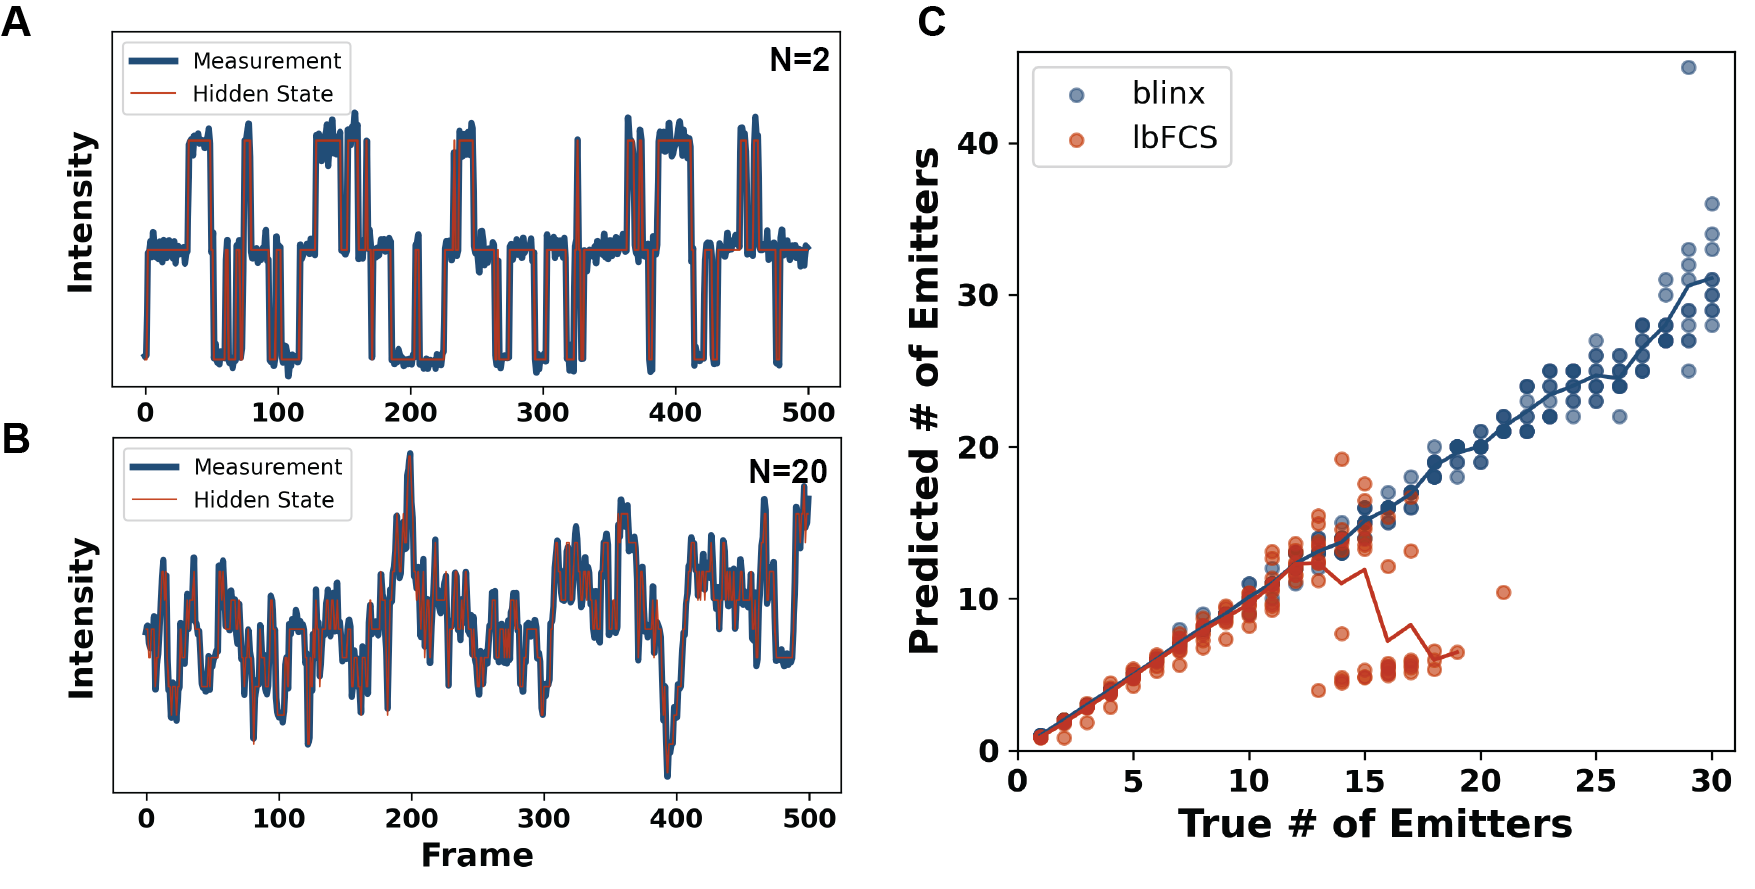
\includegraphics[width=\linewidth]{figures/comparison_lbfcs}
  \caption{A), B) simulated traces of 2 and 20 emitters, generated with experimentally plausible parameters. C) Comparison of counting results between blinx and lbFCS. Both models were applied to 10 simulated traces for each \n. Above \n = 21 lbFCS was unable to to fit the data and returned only nans. }
  \label{fig:results:comparison}
\end{figure*}

\begin{figure}[ht]
  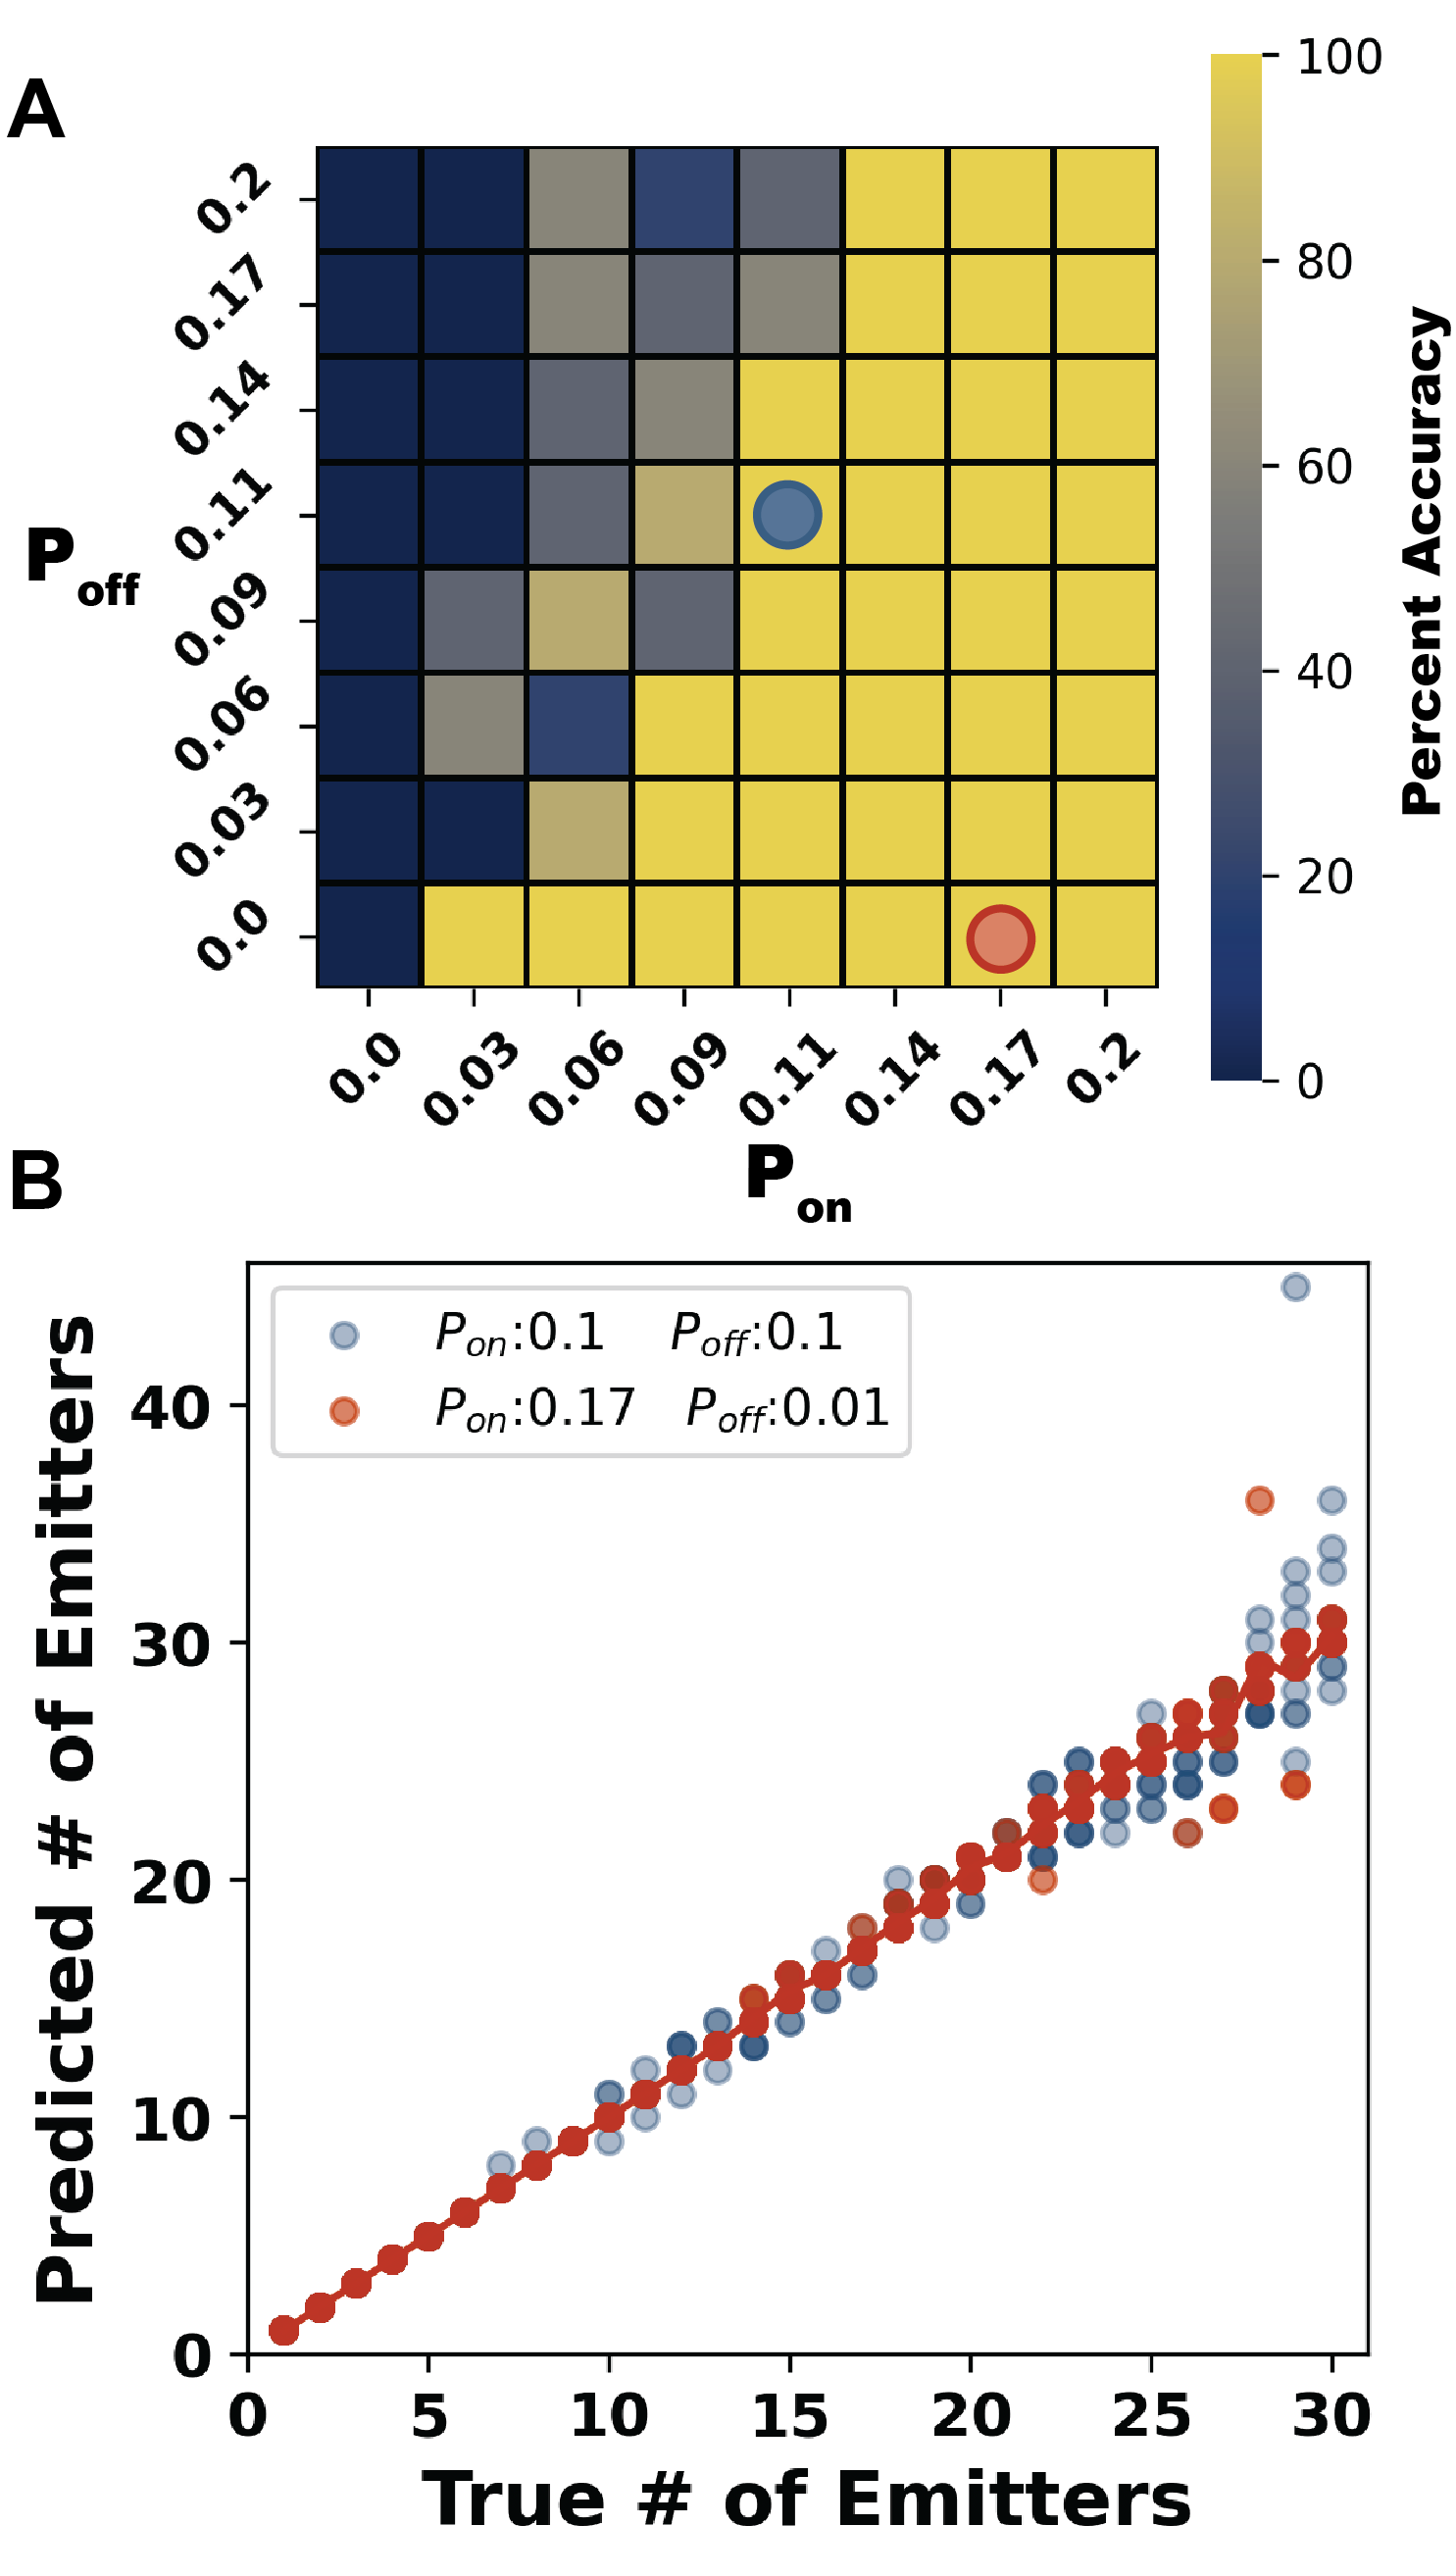
\includegraphics[width=\linewidth]{figures/kinetic_regime}
  \caption{A) The effect of kinetic parameters \pon and \poff on blinx counting accuracy of simulated traces with a \turen = 5. Accuracy increases as \pon becomes greater than \poff. B) }
  \label{fig:results:regime}
\end{figure}

\subsection{Comparison to state of the art \lbfcs}

Blinx was first benchmarked on simulated traces of 4,000 frames with known N
values between 1 and 30, and with kinetic and intensity parameters closely
matching those seen in experiments (pon=poff=0.1) (example traces shown in
\figref{fig:results:comparison}). The performance of blinx was then compared to lbFCS2 (\figref{fig:results:comparison}). 
Direct compassion to other models was not possible due to differences in
the data needed. Blinx and lbFCS2 both display good accuracy for less than 10 emitters,
however lbFCS quickly loses accuracy as the number of emitters increases and is not able to make any prediction above \truen=21. Meanwhile blinx retains a
high level of accuracy through 30 emitters. This drop off in
performance is caused by lbFCS2 reliance on a histogram-based method to
estimate the intensity of a single emitter ($\mu$). This becomes challenging
for larger numbers of emitters, as this method relies on the detection of
distinct peaks in the histogram, and specifically the identification of the \y{} =
1 peak, to accurately estimate the intensity of a single emitter. With
larger numbers of emitters however, the \y{} = 1 state becomes increasingly
less likely to be observed and harder to distinguish. Holistic methods like
blinx, on the other hand, allow inferring the intensity of a single emitter
jointly with the number of emitters active at every time-step, thus
circumventing the problem of having to observe a specific number of active emitters.

\subsection{Informing experiment}

Next it was investigated how the accuracy of blinx depends on the blinking
kinetics of the individual emitters. The emitter intensity and noise also have a
significant effect on model accuracy, but these are most heavily dependent on
microscope imaging conditions and can easily be adjusted during image
acquisition to maximize the signal to noise. Ideally the accuracy of blinx
would be invariant to different label kinetics, however some variance is
expected.

Blinx was tested on over 300 simulated traces with a \truen = 5 and ranges of
\pon and \poff values from 0.01 to 0.2 (\figref{fig:results:regime}). It was found that while blinx
displayed a high accuracy in regions where \pon $\geq$ \poff, accuracy significantly
decreased as \pon becomes much smaller than \poff. This accuracy behavior
correlates well with label occupancy, or the average number of labels
illuminated at any time. In regions where \poff  $\gg$ \pon, no matter the \truen,
the occupancy approaches 0, and the only states observed are 0 and 1 labels
illuminated. This provides very little information to the model, leading to a
significant decrease in accuracy. Interestingly, this low occupancy region is
preferred for super-resolution microscopy with literature \pon values ranging
from 0.001 to 0.05 and \poff values ranging from 0.02 to 0.36. Another
interesting observation is the increase in accuracy along the \pon = \poff
diagonal as \pon increases. As both \pon and \poff increase, transitions between
states become more common, providing more information for the model to fit.
This result also suggests that if the observation time were increased an
increase in accuracy for the low \pon = \poff region would increase.

Based on these results, it was hypothesized that accuracy could be further
increased by shifting the experimental kinetics such that \pon $\gg$ poff. Simulating
traces with \pon=0.17 and \poff= 0.01, a significantly tighter distribution
around the correct count is observed, compared to traces simulated with pon =
poff = 0.1 (Figure 2B). While it is not always possible to know the blinking
kinetics ahead of time, this finding can be used in experimental design, so as
to engineer a system so that pon \textgreater   poff and the counting potential of the model
is maximized.
